\chapter{ROC curves}
\section{Inleiding}
\begin{itemize}
	\item ROC = Receiver Operating Characteristic.
	\item Een eenvoudige manier om classifiers te evalueren.
\end{itemize}

\section{Classifiers}
\begin{itemize}
	\item Het toekennen van een klasse aan een object uit een verzameling van voorgedefinieerde klassen.
	\item Een \textbf{Binaire classifier} kent slechts twee klassen. 
\end{itemize}

\section{Binaire classifiers}
\begin{itemize}
	\item Stel twee klassen $\alpha$ en $\beta$. We zijn nu geïnteresseerd of een object in klasse $\alpha$ zit.
	\item Een \textbf{False Positive} komt voor wanneer het object de klasse $\alpha$ krijgt, terwijl hij $\beta$ is.
	\item Een \textbf{False Negative} komt voor wanneer het object de klasse $\beta$ krijgt, terwijl hij $\alpha$ is.
	\item Binaire \textbf{confusion matrix}:

	\begin{table}[h]
		\centering
		\begin{tabular}{| l | l | l |}
			\hline
		Klasse & \multicolumn{2}{l |}{Voorspelde klasse} \\
		       & positief & negatief \\
		       \hline
		positief (\#P) & \#TP & \#FN = \#P - \#TP \\
		negatief (\#N) & \#FP & \#TN = \#N - \#FP \\
		\hline
		\end{tabular}
	\end{table}

	\item De \textbf{true positive rate (TPR)} is: 
	$$TPR = \frac{\#TP}{\#P}$$
	\item De \textbf{false positive rate (FPR)} is: 
	$$FPR = \frac{\#FP}{\#N}$$
	
	\item Welke classifier is het beste?
		\begin{table}[h]
		\centering
		\begin{tabular}{| l || l | l || l | l || l | l ||}
			\hline
			Klasse & \multicolumn{2}{l ||}{Voorspelde klasse}  & \multicolumn{2}{l ||}{Voorspelde klasse} & \multicolumn{2}{l ||}{Voorspelde klasse}\\
			& positief & negatief & positief & negatief & positief & negatief \\
			\hline
			positief & {\color{green}40} & {\color{green}60} & {\color{blue}70} & {\color{blue}30} &  {\color{red}60} & {\color{red}40} \\
			negatief & {\color{green}30} & {\color{green}70} & {\color{blue}50} & {\color{blue}50}& {\color{red}20} & {\color{red}80} \\
			\hline
		\end{tabular}
		\caption{Elke kleur stelt een verschillende classifier voor die dezelfde objecten classificeert.}
		\label{table:which_classifier}
	\end{table}
	\begin{itemize}
		\item {\color{green} $TPR = 0.4, FPR = 0.3$}
		\item {\color{blue} $TPR = 0.7, FPR = 0.5$}
		\item {\color{red} $TPR = 0.6, FPR = 0.2$}
		\item Figuur \ref{fig:roc_curve} stelt deze waarden visueel voor.
		\begin{figure}
			\centering
			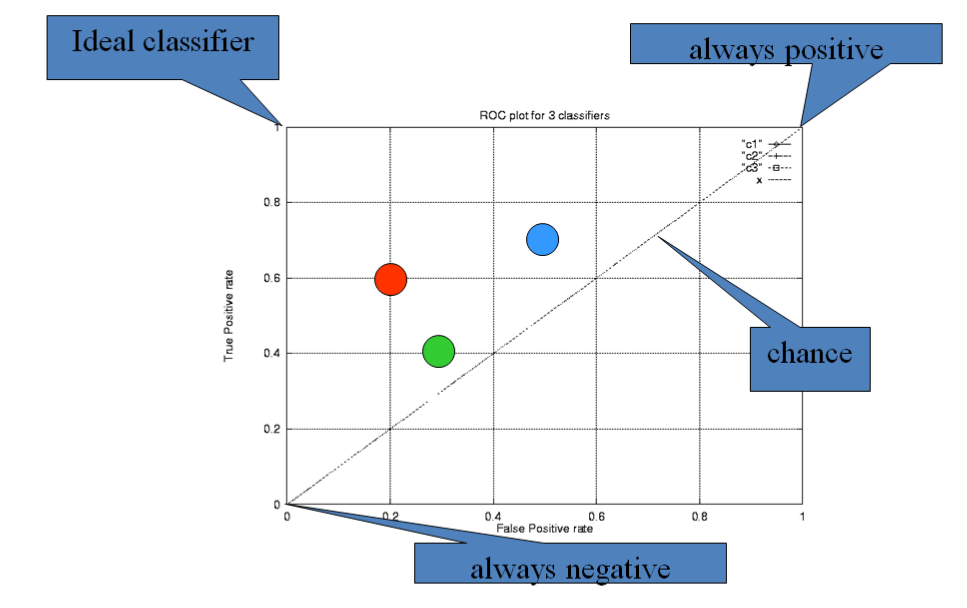
\includegraphics[width=0.5\textwidth]{roc_curve}
			\caption{De TPR en FPR van tabel \ref{table:which_classifier} gevisualiseerd.}
			\label{fig:roc_curve}
		\end{figure}
		\item De rode classifier is zeker beter dan de groene. De TPR van de rode classifier is niet beter dan de TPR van de blauwe classifier, maar de TPR/FPR verhouding is wel beter.
	\end{itemize}
	
	
	
\end{itemize}
